% ---------------------------------------------------------------
% Latex template author: Yves Peissard ypeissard@gmail.com
% ---------------------------------------------------------------

\documentclass[12pt,a4paper]{article}


%Preamble --------------------------------------------------------
%packages
%\usepackage[dvipdf]{graphicx}
\usepackage[pdftex]{graphicx}
\usepackage[a4paper,top=2.5cm,left=2.5cm,right=2.5cm,bottom=2.5cm]{geometry}
\usepackage[utf8x]{inputenc}
\usepackage{float}
\usepackage[frenchb]{babel}
\usepackage{amsmath}
\usepackage[table]{xcolor}
\usepackage{color}
\usepackage{xcolor}
\usepackage{fancyhdr}
\usepackage{url}
\usepackage{parskip}
\usepackage{wrapfig}
\usepackage{ccaption}
\usepackage{listings}
\usepackage{textcomp}
\usepackage{hyperref}
\usepackage{courier}
\usepackage{caption}
\usepackage[toc,page]{appendix}
\usepackage{hyperref}
\usepackage{breakurl}
\usepackage{bookmark}
\usepackage{tabularx}
\usepackage{subfigure}
\usepackage[xindy,toc]{glossaries}
\usepackage{setspace}
 \usepackage{enumerate}
\usepackage{pdflscape}
\usepackage{array}
\usepackage{hyperref,wasysym}
\usepackage{subfigure}



\usepackage{fancyvrb}

%do margins on even pages like in a book
\evensidemargin=-0.7cm

%generate glossary
\makeglossaries

%language selection
\selectlanguage{frenchb}

%color of links
\hypersetup{
    colorlinks,
    citecolor=black,
    filecolor=black,
    linkcolor=black,
    urlcolor=black
}




%improve figure placement
\renewcommand{\topfraction}{0.85}
\renewcommand{\textfraction}{0.1}
\renewcommand{\floatpagefraction}{0.75}



%define pagestyle
\pagestyle{fancy}
\fancyheadoffset[LE,RO]{\marginparsep}

\renewcommand{\sectionmark}[1]{\markright{#1}{}} % Lowercase sectionmark
\fancyhf{}
\fancyhead[LE,RO]{ \footnotesize \thepage}
\fancyhead[RE]{ \footnotesize Chapitre \thechapter: \leftmark}
\fancyhead[LO]{ \footnotesize \rightmark}
%\renewcommand{\footrulewidth}{0.4pt}
\renewcommand{\headrulewidth}{0.4pt}

\fancypagestyle{plain}{
\fancyhead{} % get rid of headers on first pages
\fancyfoot{} % get rid of footers on first pages
\renewcommand{\headrulewidth}{0pt} % and the line
\renewcommand{\footrulewidth}{0pt} % and the line
}
\fancyhfoffset[ER,OR,LO,LR]{0cm}


% No headers on empty pages before new chapter
\makeatletter
\def\cleardoublepage{\clearpage\if@twoside \ifodd\c@page\else
    \hbox{}
    \thispagestyle{plain}
    \newpage
    \if@twocolumn\hbox{}\newpage\fi\fi\fi}
\makeatother \clearpage{\pagestyle{plain}\cleardoublepage}

\definecolor{gray}{rgb}{0.4,0.4,0.4}
\definecolor{darkblue}{rgb}{0.0,0.0,0.6}
\definecolor{cyan}{rgb}{0.0,0.6,0.6}

%code listing
\lstset{language=Java, 
basicstyle=\ttfamily\fontsize{8}{8}\selectfont, 
showspaces=false, 
showtabs=false, 
tab= , 
keywordstyle=\bfseries, 
showstringspaces=false, 
framexleftmargin=5mm, 
frame=single, 
numbers=left,
numberstyle=\tiny, 
stepnumber=2, 
numbersep=5pt, 
breaklines=true,
xleftmargin=17pt,
captionpos=b,
escapeinside={(*@}{@*)}}


%Javascript language definition
\definecolor{darkgray}{rgb}{.4,.4,.4}

\lstdefinelanguage{JavaScript}{
  keywords={typeof, new, true, false, catch, function, return, null, catch, switch, var, if, in, while, do, else, case, break},
  ndkeywords={class, export, boolean, throw, implements, import, this},
  identifierstyle=\color{black},
  sensitive=false,
  commentstyle=\color{darkgray}\ttfamily,
  comment=[l]{//},
  morecomment=[s]{/*}{*/},
}
\lstdefinelanguage{XSD}{
    sensitive=true,
    keywords={version, encoding, targetNamespace, elementFormDefault, attributeFormDefault, xmlns:xsd, xmlns:tns, xmlns:xsi, schemaLocation, xsi:noNamespaceSchemaLocation, xsi:schemaLocation, name, type, base, value, minOccurs, maxOccurs, ref, use, default, required, mixed, fixed, itemType, memberTypes, namespace, xpath, refer},
    %otherkeywords={=},
    alsoletter={<,>,/,?,:},
    morestring=[b]{"},
    morecomment=[s]{<!--}{-->},
    morecomment=[s]{<![CDATA[}{]]>},
    keywordstyle=\color{violet},
    identifierstyle=\color{teal},
    stringstyle=\color{blue},
    commentstyle=\color{darkgray}
}
\lstdefinelanguage{XML}
{
  morestring=[b],
  morestring=[s]{>}{<},
  morecomment=[s]{!--}{--},
  stringstyle=\color{black},
  identifierstyle=\color{darkblue},
  keywordstyle=\color{cyan},
  morekeywords={xmlns,version,type}% list your attributes here
}
% Try to avoid single lines at the beginning or end of a page
\widowpenalty=300
\clubpenalty=300
%macro definitions----------------
%images
\def\EPSFIGTEXTWIDTH #1#2#3{
\begin{figure}[H]
\begin{center}	
\includegraphics[width=1\textwidth]{#1}
\end{center}			
\caption{#2}			
\label{#3}			
\end{figure}		
}

\def\EPSFIGSCALE [#1]#2#3#4{
\begin{figure}[H]
\begin{center}	
\includegraphics[scale=#1]{#2}
\end{center}			
\caption{#3}			
\label{#4}			
\end{figure}		
}

\def\EPSFIGWRAP [#1]#2#3#4 {
\begin{wrapfigure}{R}{#1\textwidth}
  \begin{center}
    \includegraphics[scale=#1]{#2}
  \end{center}
  \caption{#3}
  \label{#4}
\end{wrapfigure}
}


%equations
\def\EQ #1#2 {
\begin{equation}
#1
\label{#2}
\end{equation}
}

\def\SPLITEQ #1#2 {
\begin{equation}
\begin{split}
#1
\label{#2}
\end{split}
\end{equation}
}

%text
\def\SIDETEXT #1{
\marginpar{\begin{flushleft} \begin{footnotesize}
\textbf{\textit{#1}}
\end{footnotesize} \end{flushleft}}
}

\def\QUOTE #1{
	\begin{quote}
		\textit{''#1''}
	\end{quote}
}
\newcommand{\todo}[1]{\colorbox{red}{\color{white}:TODO: #1}}

\renewcommand{\chaptermark}[1]{ \markboth{#1}{}}
\renewcommand*\thesection{\arabic{section}}

\makeatletter
\def\cleardoublepage{\clearpage\if@twoside \ifodd\c@page\else
    \hbox{}
    \thispagestyle{empty}
    \newpage
    \if@twocolumn\hbox{}\newpage\fi\fi\fi}
\makeatother \clearpage{\pagestyle{plain}\cleardoublepage}



\newglossaryentry{ESIB}{
name={ESIB},
description={École Supérieure des Ingénieurs de Beyrouth- Faculté de l'USJ - Liban(\url{http://www.fi.usj.edu.lb/})}}
\newglossaryentry{USJ}{
name={USJ},
description={Université Saint-Joseph à Beyrouth. 5 campus dont l'FI,1873 enseignants,500 membres du personnel et
12000 étudiants(\url{http://www.usj.edu.lb/})}}

\newglossaryentry{EIA-FR}{
name={EIA-FR},
description={École d'ingénieurs et d'architectes de Fribourg- Suisse(\url{http://eia-fr.ch})}}
\newglossaryentry{GPS}{
name={GPS},
description={Le Global Positioning System (GPS) – que l'on peut traduire en français par « système de positionnement mondial » – est un système de géolocalisation fonctionnant au niveau mondial.\href{http://fr.wikipedia.org/wiki/Global\_Positioning\_System}{Plus de détail sur wikipedia} }}

\newglossaryentry{SPMP}{name={SPMP},
description={Software Project Management Plan est le doucment contenant toutes les informations concernant l'organisation d'un projet de développement de software selon la norme IEEE 1058 .\href{http://standards.ieee.org/findstds/standard/1058-1998.html}{Norme disponible à cette adresse}:\url{http://standards.ieee.org/findstds/standard/1058-1998.html}
 }
}

\newglossaryentry{Objective-C}
{name={Objective-C},
description={L'Objective-C est un langage de programmation orienté objet réflexif. C'est une extension du C ANSI, comme le C++, mais qui se distingue de ce dernier par sa distribution dynamique des messages, son typage faible ou fort, son typage dynamique et son chargement dynamique.Aujourd'hui, il est principalement utilisé pour le dévelopement d'application  Mac OS X et son dérivé iOS pou le développement iPhone,iPad,iPod.(Source wikipedia).  .\href{http://developer.apple.com/documentation/Cocoa/Conceptual/ObjectiveC/ObjC.pdf}{Référence Apple sur l'objective-c} :\url{http://developer.apple.com/documentation/Cocoa/Conceptual/ObjectiveC/ObjC.pdf}
}
}
\newglossaryentry{iOS}
{name={iOS},
description={iOS, anciennement iPhone OS, est le système d'exploitation mobile développé par Apple pour l'iPhone, l'iPod touch, et l'iPad..(Source wikipedia).\url{http://fr.wikipedia.org/wiki/IOS\_(Apple)}
}
}

\newglossaryentry{Skype}
{name={Skype},
description={Skype est un logiciel propriétaire qui permet aux utilisateurs de passer des appels téléphoniques via Internet. .   .\href{http://www.skype.com}{Site officiel} :\url{www.skype.com}
}
}

\newglossaryentry{SVN}
{name={SVN},
description={Subversion (en abrégé svn) est un système de gestion de versions, distribué sous licence Apache et BSD. \href{http://subversion.apache.org/}{Site officiel} :\url{http://subversion.apache.org/}
}
}

\newglossaryentry{Git}
{name={Git},
description={Git est un logiciel de gestion de versions décentralisée. C'est un logiciel libre créé par Linus Torvalds, le créateur du noyau Linux, et distribué sous la GNU GPL version 2.\url{ http://fr.wikipedia.org/wiki/Git}} 
}

\newglossaryentry{SRS}{name={SRS},
description={Software Requirements Specification(IEEE 830). Ce document contient la documentation concernant la spécification et l'analyse.
 }
}

\newglossaryentry{SDD}{name={SDD},
description={Software Design Description(IEEE 1016). Ce document contient la documentation concernant la conception  et l'implémentation
 }
}
\newglossaryentry{STD}{name={STD},
description={Software Test Documentation(IEEE 1016). Ce document contient la documentation concernant les tests effectué.
 }
}

\newglossaryentry{Web service}
{name={Web service},
description={Un service web est un programme informatique permettant la communication et l'échange de données entre applications et systèmes hétérogènes dans des environnements distribués. Il s'agit donc d'un ensemble de fonctionnalités exposées sur internet ou sur un intranet, par et pour des applications ou machines, sans intervention humaine, et de manière synchrone.(Source wikipedia)\url{http://fr.wikipedia.org/wiki/Service_Web}
}
}


\newglossaryentry{XCode}
{name={XCode},
description={XCode est un environnement de développement pour Mac OS X.\url{http://fr.wikipedia.org/wiki/Xcode}
}
}
\newglossaryentry{Core Data}
{name={Core Data},
description={Core Data is part of the Cocoa API in Mac OS X first introduced with Mac OS X 10.4 Tiger and for iOS with iPhone SDK 3.0.[2] It allows data organised by the relational entity-attribute model to be serialised into XML, binary, or SQLite stores. 
.(Source wikipedia)\url{http://en.wikipedia.org/wiki/Core\_Data}
}
}


%End of preamble ---------------------------------------------------



\makeglossary


\begin{document}


%Title page
\begin{titlepage}
\setlength\topmargin{0in}
\setlength\headheight{-0.3in}
\begin{center}


\includegraphics[width=1\textwidth]{../comon/logos/EIA_couleur.eps}  \\


\includegraphics[width=1\textwidth]{../comon/logos/esib_nom.jpg}  \\[0.5cm] 
\end{center}

\begin{tabular}{p{9cm} r}
\hline \\[1cm]
{ \huge {Thèse de Bachelor : } } &  \\
&  \huge \bfseries  ESIB@Pad  \\[1cm]
\hline \\[0.3cm]
 & \Large \bfseries Cahier des charges\\[1cm]
\end{tabular}

\begin{tabular}{l l l l l l}
Auteur & Elias Medawar & \\[0.1cm]
& elias.medawar@edu.hefr.ch & \\[0.5cm]
Responsables Internes  & Omar Abou Khaled & Elena Mugellini  \\[0.1cm]
&omar.aboukhaled@hefr.ch  & elena.mugellini@hefr.ch \\[0.5cm]	
Responsable externe & Dany Mezher & \\[0.1cm]
&dany.mezher@fi.usj.edu.lb   & \\[0.5cm]
Experts & Marc Wuergler  & Roland Marro   \\[.1cm]
&marc.wuergler@sunrise.ch & marror@fr.ch \\[1.5cm]	
\end{tabular}
\\
\begin{center}
\begin{tabular}{c}
Version  1 \\[0.5cm]
 {\today} \\[0.5cm]
\end{tabular}
 \end{center}
\end{titlepage}

%%%%%%%%%%%%%%%%%%%%%%%%
%%
%%  Pren1 Schlussdokument
%%  Kopf und Fusszeilen
%%  CT
%%
%%%%%%%%%%%%%%%%%%%%%%%%

\pagestyle{fancy}
  \renewcommand\headrulewidth{0.4pt}
  \fancyhf{}
  \setlength{\headheight}{35.60004pt}
%  \addtolength{\texthight}{-2*\headheight}
  \lhead{
    \protect
\includegraphics[height=35pt]{../comon/logos/EIA_ABR_Couleur.eps}
  }
  \rhead{
    ESIB@Pad: Rapport release 0.3\\
   Elias Medawar\\
  }
  \cfoot{
    \thepage
  }
\fancypagestyle{plain}{
  \renewcommand\headrulewidth{0.4pt}
  \fancyhf{}
  %\addtolength{\headheight}{\baselineskip}
  \lhead{
    \protect
\includegraphics[height=32pt]{../comon/logos/EIA_ABR_Couleur.eps}
  }
  \rhead{
    Rapport de release\\
    0.3\\
  }
  \cfoot{
  }
}
\fancypagestyle{empty}{
  \renewcommand\headrulewidth{0pt}
  \fancyhf{}
  %\addtolength{\headheight}{\baselineskip}
  \lhead{
  }
  \cfoot{
  }
}


%Table of contents page
\thispagestyle{empty}


\begin{spacing}{0.9}
\renewcommand\contentsname{Table des matières}
\tableofcontents
\thispagestyle{empty} 

\end{spacing}

\vspace{1cm}
\begin{large}
\textbf{Évolution de ce  document\\}
\end{large}
\begin{tabular}{|c|l|l|l|}
\hline  Rev &  Date &  Auteur & Remarque \\ 
\hline  1 &  02.06.2011 & Medawar  & Création de la premières version du SRS. \\ 
\hline  2 &  13.06.2011 & Medawar  & Ajouts des éléments pour la release 0.1  . \\ 
\hline  3 &  22.06.2011 & Medawar  & Ajouts des éléments nécessaire pour la release 0.2. \\ 
\hline  4 &  04.07.2011 & Medawar  & Ajouts des éléments nécessaire pour la release 0.3. \\ 

\hline 
\end{tabular} 

\newpage

%CAHIER DES CHARGES
	\section{Introduction}
	Ce chapitre regroupe toutes les informations relatives à la gestion du projet et du processus de développement.Ce chapitre est mis à jour régulièrement afin de permettre à tout moment d'avoir un aperçu de l'avancement du projet.

\section{Organisation}
	L'annexe A (/Documentation/Annexes/A\_Directives) contient les directives qui ont été distribuées au début du projet. Ces directives sont la ligne directrice concernant l'organisation du projet et sont complétées par ce document.
	Le cahier des charges de l'annexe G a été créé et validé en début de projet, il est la référence en ce qui concerne les objectifs à atteindre. 
	
	\subsection{Séances}
	\begin{itemize}
		\item Des séances hebdomadaires seront effectuées avec M. Dany Mezher, le responsable externe .
		\item Une séance est tenue si possible toute les 2-3 semaines via Skype avec Mme Mugellini et M. Abou Khaled, les responsables internes.
		\item Au moins une séance est organisée avec les experts M. Roland Marro et M. Marc Wuergler via Skype.
	\end{itemize}
	\subsection{Site internet}
		Un site internet est mis en ligne et il est disponible à l'adresse suivante: \url{https://forge.tic.eia-fr.ch/projects/esibpad} \\
		Mme Mugellini et M. Abou Khaled peuvent utiliser leur login AII pour accéder aux données.\\
		Pour les autres personnes, des comptes ont été créés par le service informatique de l'école. Les comptes sont valides jusqu'au 31.12.2011. \\[1cm]
		
		\begin{table}[H]
			\centering
			\begin{tabular}{|c|c|}
				\hline M.Dany Mezher &  \\ 
				\hline   Username : &  dany.mezher   \\ 
				\hline   Password : & voir mail     \\ [0.2cm]
				\hline M.Marc Wuergler & \\ 
				\hline   Username : &  marc.wuergler  \\ 
				\hline   Password : & voir mail \\ [0.2cm]
				\hline M.Roland Marro &  \\ 
				\hline   Username :&  roland.marro  \\ 
				\hline   Password : & voir mail     \\
				\hline
			\end{tabular} 
			\caption{\label{tab.login}Données de login pour les personnes externe à l'EIA-FR}
		\end{table}
	
		Le site contiendra:
	 	\begin{itemize}
	 		\item le journal de bord :\url{https://forge.tic.eia-fr.ch/projects/esibpad/wiki}
			\item Les PVs :\url{https://forge.tic.eia-fr.ch/projects/esibpad/documents} 
			\item La documentation sous format PDF:\url{https://forge.tic.eia-fr.ch/projects/esibpad/documents} 
		\end{itemize}
	\subsection{Communication}
		Le moyen de communication principal est l'e-mail.\\
		\begin{table}[H]
			\begin{tabular}{|l|l|l|}
				\hline  Nom & email  & Téléphone [Fixe, Mobile]  \\ 
				\hline M. Würgler Marc & marc.wuergler@sunrise.ch  & +41 26 660 03 04, +41 78 609 49 44  \\ 
				\hline M. Marro Roland & marror@fr.ch  & +41 26 305 31 61  \\ 
				\hline M. Dany Mezher	& dany.mezher@fi.usj.edu.lb & +961 142 134 1,+961 700 100 30  \\ 
				\hline Mme Elena Mugellini & elena.mugellini@hefr.ch &  +41 26 429 68 70\\ 
				\hline M. Omar Abou Khaled & omar.aboukhaled@hefr.ch  &  +41 26 429 65 89\\ 
				\hline M. Elias Medawar & elias.medawar@edu.hefr.ch  &  +961 712 900 72, +41 764 090 330\\ 
				\hline 
			\end{tabular} 
			\caption{Résumé des adresses e-mail et des numéros de téléphone.}			
		\end{table}
	
		Des rendez-vous pour des vidéo-conférences seront organisés à l'aide de \gls{Skype}.
\section{Planification}
	\subsection{Plan global}
	 \EPSFIGTEXTWIDTH{../comon/figures/timeLineDetail.pdf}{Vue détaillée du planning du projet}{planGlobDet}

	 \subsection{Description des jalons}

		 \begin{longtable}{|c|l|p{10cm}|}

		 \hline  \textbf{Nom} & \textbf{Date}  & \textbf{But à atteindre}  \\ 
		 \endfirsthead
		  \multicolumn{3}{|r|}{{suite de la page précédente}} \\ \hline
		\hline  \textbf{Nom} & \textbf{Date}  & \textbf{But à atteindre}  \\ 
		 \endhead
		  \multicolumn{3}{|r|}{{Suite à la page suivante}} \\ \hline
		 \endfoot
		 \endlastfoot
		 \hline  Milestone 1 & 03.06.11  & 
		 	\begin{itemize}
		 	 		\item Le cahier des charges est établi et validé.
		 			\item La première version du \gls{SPMP} est rédigée.
		 	\end{itemize}   \\ 
		 \hline  Milestone 2 & 10.06.11  & 
		 	\begin{itemize}
		 	 		\item Pouvoir déployer une simple application sur l'iPhone et l'iPad.
		 			\item Un environnement de développement local est mis en place, avec des Web Services de test ainsi que des données de test.
		 	\end{itemize}   \\ 
	 	 \hline  Release 0.1 & 17.06.11  & 
		 	\begin{itemize}
		 	 		\item La page d'accueil de l'application avec les différents menus est réalisée.
		 			\item La page de paramètres de l'application est réalisée.
		 	\end{itemize}   \\ 
	 	 \hline  Release 0.2 & 01.07.11  & 
		 	\begin{itemize}
		 	 		\item Afficher la carte du campus.
		 	 		\begin{enumerate}[a)]
	 	 				\item La position actuelle de l'utilisateur sera détectée à l'aide du \gls{GPS} de l'appareil et affichée sur la carte.
	 	 				\item L'utilisateur peut, à l'aide de la fonction ''chercher'' : trouver l'emplacement d'une salle ou le bureau d'une personne.
	 	 				\item Les informations de la carte sont enregistrées sur le serveur et peuvent être mises à jour à tout moment. Un système de cache évite de recharger la carte à chaque visite.
	 	 			\end{enumerate}
		 	\end{itemize}   \\ 
		 \hline  Release 0.3 & 13.07.11  & 
 		 	\begin{itemize}
 		 	 		\item Permettre de consulter les nouvelles du campus.
	 		 	 	\begin{enumerate}[a)]
	 		 	 			\item Si une nouvelle est liée à un lieu, permettre de l'afficher facilement sur la carte.
	 		 	 		\end{enumerate}
 		 	\end{itemize}   \\
		\hline  Release 0.4 & 22.07.11  & 
				\begin{itemize}
 		 	 		\item Permettre l'accès à l'annuaire de l'université. 
	 		 	 	\begin{enumerate}[a)]
		 	 				\item Quand on clique sur un numéro de téléphone, l'appel est lancé.
		 	 				\item Quand on clique sur une adresse mail, la fenêtre d'envoi de mail de l'appareil est ouverte.
		 	 			\end{enumerate}
 		 	\end{itemize}   \\
		\hline  Release 0.5 & 03.08.11  & 
 		 
 	 		 	\begin{itemize}
 	 		 	 		\item Permettre aux professeurs et aux étudiants d'afficher leurs horaires.
 		 		 	 	\begin{enumerate}[a)]
 		 		 	 			\item Quand on clique sur un cours, l'emplacement de ce dernier est affiché sur la carte.
 		 		 	 			\item L'utilisateur peut sauvegarder son horaire sur l'appareil pour un accès offline.
 		 		 	 		\end{enumerate}
 	 		 	\end{itemize}   \\ 
	 	\hline  Release 0.6 Version 1 & 03.08.11  & 
 		 	\begin{itemize}
 		 	 		\item Permettre aux étudiants de consulter le résultat des examens. \textbf{Cet objectif est conditionné par l'accord de l'administration et du service informatique de l'\gls{ESIB}.}
 		 	\end{itemize}   \\  
	 	\hline  Milstone 3 &  19.08.11 &
	  		 	\begin{itemize}
	  		 	 		\item L'application est prête à être publiée sur l'App store.
	  		 	 		\item La documentation est finie.
	  		 	 		\item La présentation finale est prête.
	  		 	\end{itemize}   \\  
		 \hline 
		\caption{\label{tab.DescMils}Description des jalons. Les date de releases sont considérées comme des jalons.}  \\
	 \end{longtable} 

	 \begin{landscape}
	 	 \subsection{Planification détaillé}
		 \begin{figure}[H]
			 \begin{center}	
				 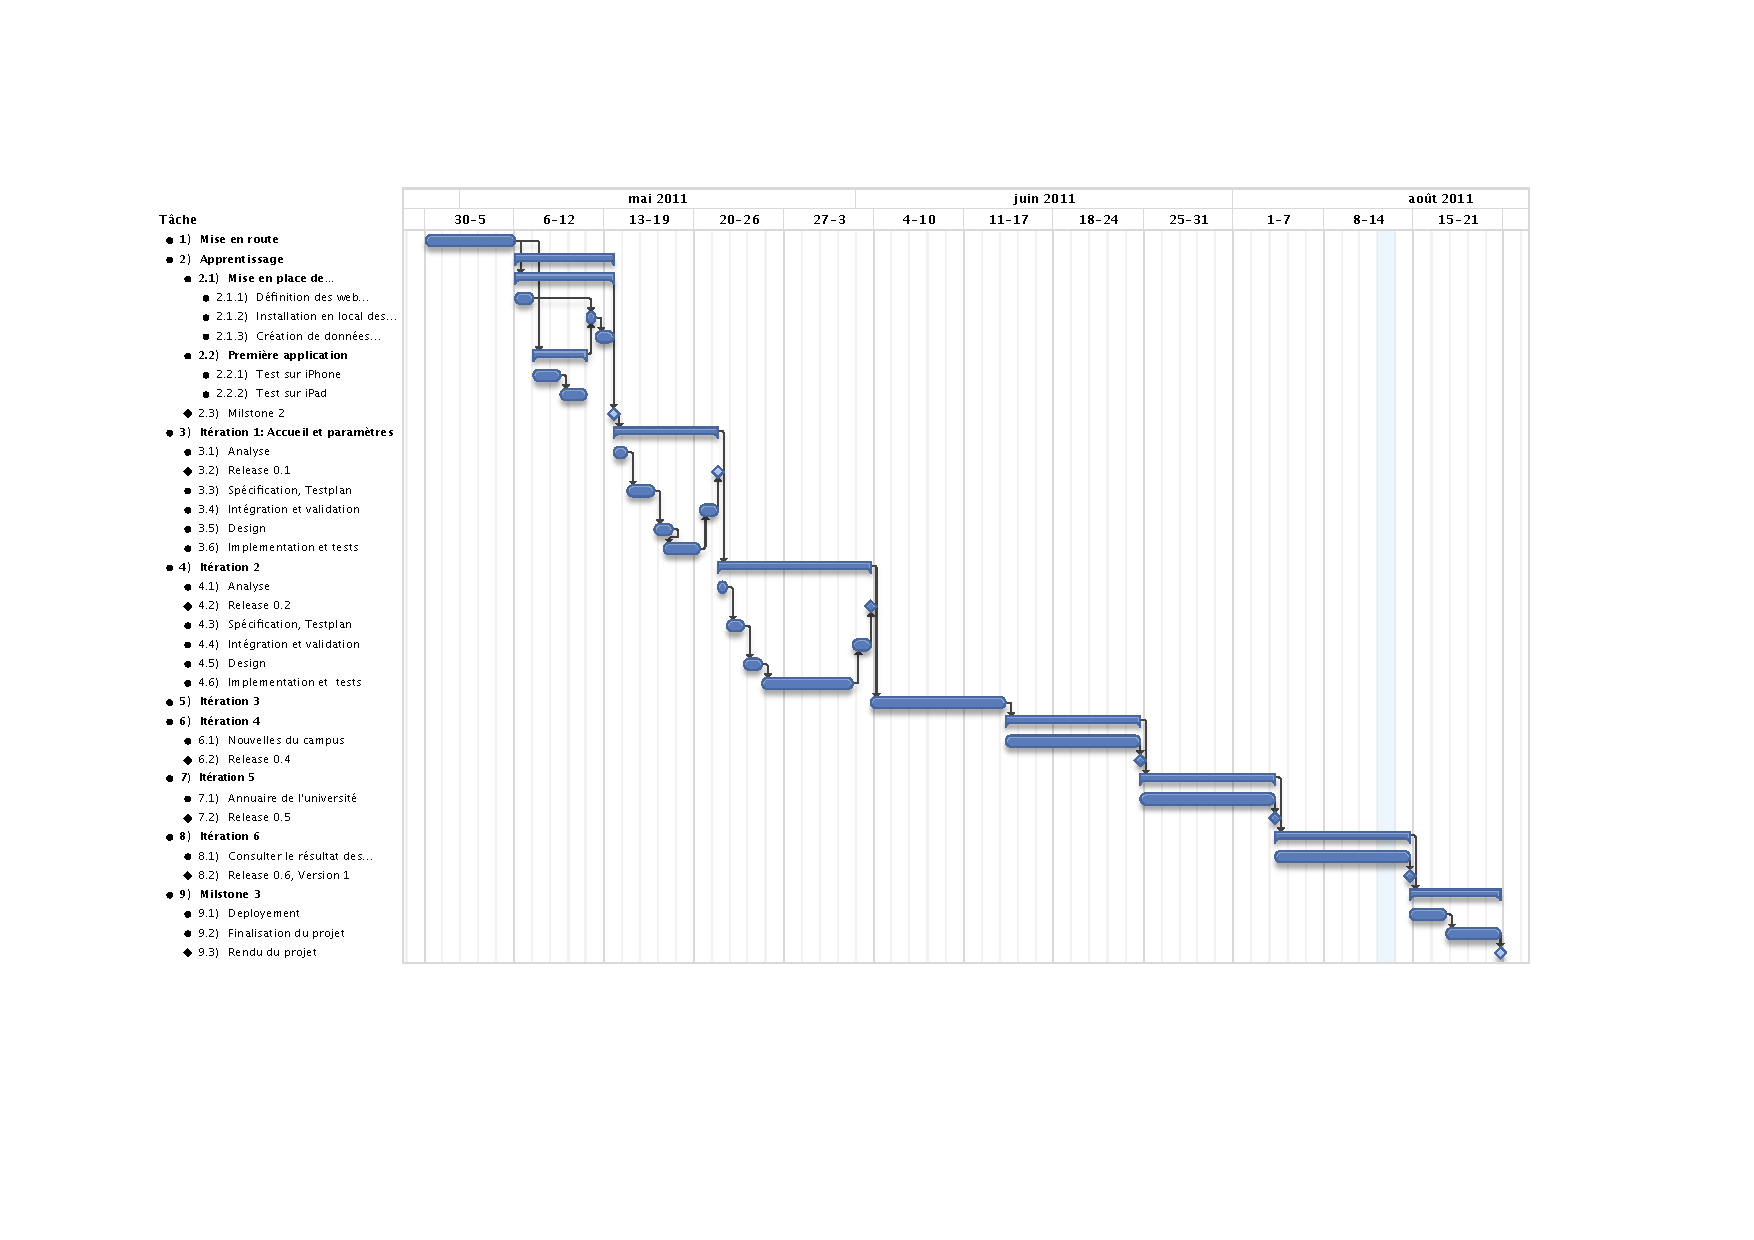
\includegraphics[height=0.8\textwidth]{../comon/figures/planningV3.pdf}
				 \end{center}			
				 \caption{Vue globale du planning du projet avec les milestones}			
				 \label{planV1}			
		 \end{figure}	
	 \end{landscape}
	 La planification détaillée de chaque itération n'est pas  faite, elle sera faite au début de chaque itération si besoin est. Etant seul à travailler sur les tâches et vu que les itérations sont courtes, une planification plus détaillée est inutile. En début d'itération, une liste de tâches à faire (TODO) est faite avec une estimation du temps nécessaire pour atteindre l'objectif. Ce fonctionnement s'approche de la méthode de travail Scrum.
	  
\section{Processus technique}
Sur la Figure~\ref{planGlobDet} nous pouvons voir que nous allons travailler par itérations. Voici une définition plus détaillée de ce que l'on entand par itération 
	 \EPSFIGTEXTWIDTH{../comon/figures/vModel.pdf}{Illustration du modèle de développement en V qui est appliqué à chaque itération. }{vModel}
\textit{``Le modèle du cycle en V a été imaginé pour pallier au problème de réactivité du modèle en cascade. Ce modèle est une amélioration du modèle en cascade qui permet, en cas d'anomalie, de limiter un retour aux étapes précédentes. Les phases de la partie montante doivent renvoyer de l'information sur les phases en vis-à-vis lorsque des défauts sont détectés afin d'améliorer le logiciel.
De plus, le cycle en V met en évidence la nécessité d'anticiper et de préparer dans les étapes descendantes les « attendus » des futures étapes montantes : ainsi les attendus des tests de validation sont définis lors des spécifications, les attendus des tests unitaires sont définis lors de la conception, etc.
Le cycle en V est devenu un standard de l'industrie du développement de logiciel et de la gestion de projet depuis les années 1980. ``}\cite{wikiV}

Ainsi cette approche sera nommée une itération et elle sera répétée à chaque release pour arriver au but qui a été fixé.
\section{Gestion des risques}
Les divers risques qui mèneraient à un échec du projet sont résumés ici. Le but est de mettre à jour les risques régulièrement, et de faire qu'ils diminuent au plus vite. 
	\subsection{État le 01/06/2011  }
	\begin{table}[H]
	\begin{tabular}{|l|p{6cm}|l|l|l|p{6cm}|}
		\hline  Nr. & Risque & P  & DC & I & Mesure \\ 
		\hline  T1 & Le peu d'expérience dans le développement \gls{Objective-C} induit en erreur(sous estimation de la charge de travail, mauvaise architecture,etc) lors de la prise de décisions importantes au début du projet & 3 & 3 & 9 & Discuter les décisions avec des personnes ayant de l'expérience dans le domaine, prendre le temps d'apprendre les bases de l'\gls{Objective-C} au début du projet et prévoir une tâche simple pour la première itération.  \\ 
		\hline  T2 & Les services web ne sont pas encore opérationnels et peuvent retarder l'avancement du projet & 3 & 3 & 9 & Prévoir un environnement de développement en local avec des Web Services de test indépendants.  \\ 
		\hline  N1 & La méthodologie de travail au sein de l' \gls{EIA-FR} diffèrent trop de celle de l'\gls{ESIB}  et les méthodes ne conviennent pas à l'une ou l'autre partie.  & 1 & 2 & 2 & Organiser régulièrement des séances pour valider les décisions.  \\ 
		\hline  N2 & Sous-estimation de la charges de travail, dépassement du temps mis à disposition.  & 2 & 2 & 4 & Travailler par itération et se baser sur l'expérience acquise lors des itérations précédentes pour bien planifier les suivantes.Ne pas rester bloqué sur une étape sans demander de l'aide.  \\ 
		
		\hline 
	\end{tabular} 
	\caption{ Risques identifié au lancement du projet.\\ Légende :\\
Tx = Risque technique\\
Nx = Risque non technique\\
P = Probabilité  (1 peu probable / 3 très probable)\\ 
DC = Dégât et conséquence (1 peu / 3 grave)\\
I =  Importance ([1-2 petite][3-4 moyenne][5-9 sérieux])(P*DC)
}
	\end{table}
Les risques T1 et T2 qui sont d'une grande importance ont été pris en considération pour la planification.
	\subsection{État le 04/07/2011  }
	\begin{table}[H]
	\begin{tabular}{|l|p{6cm}|l|l|l|p{6cm}|}
		\hline  Nr. & Risque & P  & DC & I & Mesure \\ 
		\hline  {\color{green}T1} & Le peu d'expérience dans le développement \gls{Objective-C} induit en erreur(sous estimation de la charge de travail, mauvaise architecture,etc) lors de la prise de décisions importantes au début du projet & 2 & 3 & 6 & Ce risque à diminuer suite à l'expérience acquise durant la première itération.  \\ 
		\hline  {\color{green}T2} & Les Web Services ne sont pas encore opérationnels et peuvent retarder l'avancement du projet & 1 & 3 & 3 & Diminution suite à la création d'un environnement de test stable et contrôlable. Une première version des web services a été mis en place par le service informatique de l'\gls{USJ}  .  \\ 
		\hline  N1 & La méthodologie de travail au sein de l' \gls{EIA-FR} diffèrent trop de celle de l'\gls{ESIB}  et les méthodes ne conviennent pas à l'une ou l'autre partie.  & 1 & 2 & 2 & Organiser régulièrement des séances pour valider les décisions.  \\ 
		\hline  {\color{red}N2} & Sous-estimation de la charges de travail, dépassement du temps mis à disposition.  & 3 & 2 & 6 & Suite au retard pris lors de la première itération ce risque augmente.  \\ 
		
		\hline 
	\end{tabular} 
	\caption{ Risques après la première itération.\\ Légende :\\
Tx = Risque technique\\
Nx = Risque non technique\\
P = Probabilité  (1 peu probable / 3 très probable)\\ 
DC = Dégât et conséquence (1 peu / 3 grave)\\
I =  Importance ([1-2 petite][3-4 moyenne][5-9 sérieux])(P*DC)
}
	\end{table}
Les probabilités des risques T1 et T2  ont diminué après le premier mois de développement tandis que celle du risque N2 a augmenté. On peut constater que globalement les risques diminuent. Il faut travailler sur la planification pour diminuer au plus vite le risque N2.

	\subsection{État le 08/08/2011  }
	\begin{table}[H]
	\begin{tabular}{|l|p{6cm}|l|l|l|p{6cm}|}
		\hline  Nr. & Risque & P  & DC & I & Mesure \\ 
		\hline  {\color{green}T1} & Le peu d'expérience dans le développement \gls{Objective-C} induit en erreur(sous estimation de la charge de travail, mauvaise architecture,etc) lors de la prise de décisions importantes au début du projet &0 & 3 & 0 & Ce risque peut être considéré nul vu l'expérience acquise jusq'à présent   \\ 
		\hline  {\color{green}T2} & Les Web Services ne sont pas encore opérationnels et peuvent retarder l'avancement du projet & 1 & 1 & 1 & aucun changement.  \\ 
		\hline  \color{green}N1 & La méthodologie de travail au sein de l' \gls{EIA-FR} diffèrent trop de celle de l'\gls{ESIB}  et les méthodes ne conviennent pas à l'une ou l'autre partie.  & 0 & 2 & 0 & Le système des 2 écoles n'est pas incompatibles et la manière de travail convient aux 2 selon les différentes séance organisées et les commentaires émis. .  \\ 
		\hline  {\color{green}N2} & Sous-estimation de la charges de travail, dépassement du temps mis à disposition.  & 1 & 2 & 2 & Des heures de travail supplémentaires ont été faites pour rattraper le retard et on est dans le temps selon la planification.  \\ 
		\hline 
	\end{tabular} 
	\caption{ Risques après la première itération.\\ Légende :\\
Tx = Risque technique\\
Nx = Risque non technique\\
P = Probabilité  (1 peu probable / 3 très probable)\\ 
DC = Dégât et conséquence (1 peu / 3 grave)\\
I =  Importance ([1-2 petite][3-4 moyenne][5-9 sérieux])(P*DC)
}
	\end{table}
A cette étape du projet, on peut dire que les risques d'échec sont quasi nuls, il faut toutefois garder un rythme de travail assez soutenu pour parvenir au bout à temps.  

\section{Gestion des configurations}
Afin de garder des traces de l'évolution du projet, des versions des sources des documents seront sauvegardées sur un serveur \gls{SVN}. La version courante du projet est hébergée à l'adresse suivante:  \sout{\url{http://esibpad.googlecode.com/svn/trunk/}} \url{https://github.com/eia-fr/ESIB_PAD/}\footnote{Suite à des problèmes technique rencontré pour communiquer via SVN, le protocole \gls{Git} est utilisé à partir de la release 2} . Les releases seront stockées  à l'emplacement suivant: \sout{\url{http://esibpad.googlecode.com/svn/tags/}} \url{ https://github.com/eia-fr/ESIB_PAD/tree/} 

	 \EPSFIGTEXTWIDTH{../comon/figures/config0_5}{Compatibilité entre composants et versions du logiciel. Les traits continus représentent une compatibilité à 100 \%, les traits traitillés représentent une compatibilité partielle.}{config0_5}
	 
\textbf{GCCalendar} : est un composant externe open source qui permet d'afficher un calendrier pour une journée.\cite{gcCalendar} La version  v 1.1.1 est une adaptation de la version officielle faite par moi-même pour mieux répondre aux besoins du projet et qui permet l'affichage du composant dans une partie de l'écran pour l'iPAD et non uniquement en plein écran sur iPhone.Cette adaptation prend aussi en charge le changement de journée grâce au mouvement ''glisser'' du doigt sur l'écran. Cette version a été transmise à l'auteur pour ainsi faire évoluer ce composant.

\section{Gestion de la documentation}
 La documentation sera conçue selon les différentes normes IEEE sur la documentation de software. Elle contiendra notamment les documents suivants:

\begin{enumerate}
	\item \gls{SPMP} - Software Project Management Plan (IEEE 1058).  Ce document contient toutes les informations concernant l'organisation d'un projet de développement de software . Il a pour but de rendre transparente l'organisation du projet et aide les chefs de projets à avoir un aperçu global de l'état d'avancement.
	\item \gls{SRS} - Software Requirements Specification(IEEE 830). Ce document contient la documentation concernant la spécification et l'analyse.
	\item \gls{SDD} - Software Design Description(IEEE 1016). Ce document contient la documentation concernant la conception  et l'implémentation.
	\item \gls{STD} - Software Test Documentation(IEEE 1008). Ce document contient la documentation concernant les tests effectués.
\end{enumerate}	

Il est important d'indiquer que la documentation ne sera pas complètement conforme à la norme, car cela représenterait une trop grande charge de travail. En effet, les différentes normes sont très complètes et plusieurs chapitres ne sont pas adaptés à notre projet. La variante de documentation qu'on utilise est inspirée de celle utilisé par la ''Hochschule Luzern '' (école d'ingénieurs Suisse alémanique dans laquelle j'ai eu l'occasion d'étudier durant 6 mois).

Les documents seront regroupés en chapitre pour former le rapport final du projet.

\section{Gestion des finances}
Ce travail fait partie du processus de formation et ne traite pas en détail de l'aspect financier. Cependant voici tout de même quelques informations que l'on peut citer:
\subsection{Ressources humaines}
\begin{itemize}
	\item 1 futur ingénieur HES  à 100\%  soit 40 heures par semaine durant 12 semaines. Une bourse est versée par  l'\gls{EIA-FR} à l'étudiant pour le transport jusqu'au Liban ainsi que le logement sur place. 
\end{itemize}
\subsection{Ressources matérielles}
\begin{itemize}
	\item 1 iPad2 et 1 iPhone 4  mis à disposition par l'\gls{EIA-FR}
	\item local de travail mis à disposition par l'\gls{ESIB}
\end{itemize}



%Examples

%  1.Figures ------------------------------------------------------------------------------------------
%    \EPSFIGTEXTWIDTH{source}{caption}{label}     sets eps image size to textwidth
%
%    \EPSFIGSCALE[0.5]{source}{caption}{label}    sets eps image size to 0.5 * the original size
%
%    \EPSFIGWRAP [0.5]{source}{caption}{label}    sets size of a wraped eps image to 0.5 * the textsize
%
%
%  2.Equations ----------------------------------------------------------------------------------------
%    \EQ{x = 1}{label}
%
%    \SPLITEQ{                                    used for longer calculations
%    1 \cdot 1 & = 1\\                            the & is the alignment character
%    2 \cdot 2 \cdot 2 & = 8
%    }{label}
%
%
%  3.Code listing --------------------------------------------------------------------------------------
%    \begin{lstlisting}[label=samplecode,caption=A sample]   simple listing. configure language in config.tex.
%        for (int i = 0; i < 10; i++) {                      default language is java
%            // increment p  (*@\label{timer-1}@*)
%            p++ = i;
%        }
%    \end{lstlisting}
%
%    \lstinputlisting[label=samplecode,caption=A sample]{listings/Graph.java}   list a whole file
%
%
%  3.Bibliography reference
%    \cite{Chaiken1995}
%
%
%  4.Text outside of margin
%    \SIDETEXT{text}
%
%
%  5. Glossary Entry
%  \gls{Latex}
%  \glspl{Latex}    (pl for plural)

%   PUT YOUR CONTENTS HERE  -----------------------------------------------------------------------------------



%Bibliography: Use JabRef to manage your bibliography: http://jabref.sourceforge.net/
%\clearpage
%	\addcontentsline{toc}{chapter}{Referenzen}


\newpage

%\renewcommand{\bibname}{Referenzen}

%\begin{flushleft}
%\bibliography{./bibliography/references}
%\end{flushleft}

%\bibliographystyle{plain}



%Glossary
\printglossary

%appendices
%\newpage
%\pagestyle{plain}
%\begin{appendices}
%	\appendix

%\end{appendices}


\end{document}
